% !TeX program = lualatex
% ================================================================
% Chinese (Traditional) Parallel Text Version of IntroducingIndicesAndRoots
%
% Generated by the server using the following settings:
%
%   language            Chinese (Traditional) (zht)
%   text direction      left to right
%   font                Noto Sans CJK TC
%   fallback font       Noto Serif
%   built from          latex/worksheets/indices/introducingIndicesAndRoots.tex
%   vocabulary key      latex/worksheets/indices/introducingIndicesAndRoots/L2/zht/introducingIndicesAndRoots_chinesetraditionalKey.tex
%   tier 3 vocabulary   green   RGB 0 128 0
%   English text        black   RGB 0 0 0
%   Chinese (Traditional) textpurple  RGB 112 48 160
%   layout macros       version 3
%
% Please don't edit any information in this comment block - the server
% compares it against the current settings and rebuilds this file when
% they differ, so changes here would be overwritten. However, feel free
% to make updates to the LaTeX below if you want to edit it.
% ================================================================

\documentclass[12pt,a4paper]{article}
% ================================================================
% Copied from the English sheet this was translated from, so that
% anything it sets up for itself still works here
% ================================================================
\usepackage[a4paper,top=12mm,bottom=14mm,left=15mm,right=15mm]{geometry}
\usepackage[T1]{fontenc}
\usepackage{amsmath}
\usepackage{amssymb}
\usepackage{cancel}
\usepackage{enumitem}
\usepackage{multicol}
\usepackage{array}
\usepackage{tikz}
\usepackage[most]{tcolorbox}
\usetikzlibrary{arrows.meta}

% ================================================================
% An introduction to indices and roots.
%
% A first sheet on index notation that also builds on algebraic
% notation and on simplifying fractions. Indices are met first with
% integers and decimals, through a match-up of calculations and their
% answers, and then in context through the area of a square and the
% volume of a cube, where the root appears as the operation that
% undoes the index.
%
% The sheet then moves to algebraic variables, writing repeated
% multiplications such as a x a x a over b x b in index form and back
% again. Cancelling a factor found in both the numerator and the
% denominator is taught with integers first, then with a mix of
% integers and variables, and is then used on fractions written with
% indices in a second match-up.
%
% The extension uses the same cancelling on factorials, where most of
% the factors divide out, then asks what happens to powers and roots
% of negative numbers, and ends on the tesseract, the four-dimensional
% shape after the cube, whose corners, hypervolume and edges are all
% counted by powers of 2. Answers are on the last page.
%
% The sheet is written on, so every question is followed by a working
% area. The \newpage commands in the body are placed so that no
% question is split across the fold.
% ================================================================

\pagestyle{empty}
\linespread{1.15}\selectfont
\setlength{\parskip}{5pt}
\setlist[enumerate,1]{label=\textbf{Q\arabic*.}, leftmargin=*, itemsep=10pt, topsep=6pt, parsep=4pt}
\setlist[enumerate,2]{label=(\alph*), leftmargin=*, itemsep=8pt, topsep=5pt, parsep=3pt}
\setlength{\multicolsep}{4pt}
\setlength{\parindent}{0pt}

\newcommand{\ansline}[1][2.2cm]{\underline{\hspace{#1}}}
% A short gap for a single number, sized to sit inside a line of maths.
\newcommand{\gap}{\underline{\hspace{0.7cm}}}
% A gap for a number that is written as an index, or on the top or the
% bottom of a fraction. An underline sits too low to be read as an
% index, so a faint dotted box marks where the number is written. The
% size is given in points so that the box does not shrink away when it
% is set as an index.
\newcommand{\boxgap}[1][9pt]{\tikz[baseline=-0.8pt]\draw[gray!60,densely dotted,thick]
  (0,0) rectangle (#1,#1);}

% A worked example: the method shown in full before it is practised.
% The boxes are tinted only faintly, and their title bars are pale with
% coloured text rather than solid, so that the sheet is cheap to print.
\newtcolorbox{wex}[1]{colback=blue!1,colframe=blue!45!black,boxrule=0.6pt,
  colbacktitle=blue!8,coltitle=blue!50!black,
  left=6pt,right=6pt,top=4pt,bottom=5pt,
  title={\bfseries\small Worked example: #1},fonttitle=\small,
  toptitle=1pt,bottomtitle=1pt}

% The idea a section is built on, stated once and boxed.
\newtcolorbox{keyidea}{colback=orange!2,colframe=orange!60!black,boxrule=0.6pt,
  left=6pt,right=6pt,top=4pt,bottom=4pt}

% The notation for a section, set out so that it can be found again
% from anywhere on the sheet.
\newtcolorbox{notation}[1]{colback=green!1,colframe=green!35!black,boxrule=0.9pt,
  colbacktitle=green!10,coltitle=green!30!black,
  left=8pt,right=8pt,top=5pt,bottom=5pt,
  title={\bfseries Notation: #1},fonttitle=\normalsize,
  toptitle=2pt,bottomtitle=2pt}

% A warning about a mistake that is easy to make.
\newtcolorbox{warning}{colback=red!2,colframe=red!55!black,boxrule=0.6pt,
  left=6pt,right=6pt,top=4pt,bottom=4pt}

% The section headings, kept tight so the parts do not eat the page.
\newcommand{\heading}[1]{%
  \vspace{2pt}
  {\color{blue!45!black}\rule{\linewidth}{1pt}}\\[1pt]
  {\large\bfseries #1}\\[-6pt]
  {\color{blue!45!black}\rule{\linewidth}{0.4pt}}
  \vspace{2pt}}
\newcommand{\parttitle}[2]{\heading{Part #1: #2}}

% ----------------------------------------------------------------
% A match-up: calculations in a numbered column on the left, answers in
% a lettered column on the right, with a gap between them for the lines
% pupils draw. The answers are deliberately out of order.
% \matchup[<row spacing>][<column gap>]{<left items>}{<right items>}
% Each item is written inside braces so that it counts as one item.
\newcommand{\mletter}[1]{\ifcase\numexpr#1\relax\or A\or B\or C\or D\or E\or
  F\or G\or H\or I\or J\fi}
\NewDocumentCommand{\matchup}{O{1.1} O{7.2} +m +m}{%
\par\vspace{2pt}\noindent\hfil
\begin{tikzpicture}[mbox/.style={draw=blue!45!black,rounded corners=3pt,thick,
    fill=white,minimum width=2.9cm,minimum height=0.9cm,inner sep=3pt}]
  \foreach [count=\i from 1] \l in {#3} {%
    \node[mbox] (mL\i) at (0,{-#1*\i}) {\l};
    \node[font=\small\bfseries,anchor=east] at ([xshift=-5pt]mL\i.west) {\i.};}
  \foreach [count=\j from 1] \r in {#4} {%
    \node[mbox] (mR\j) at (#2,{-#1*\j}) {\r};
    \node[font=\small\bfseries,anchor=west] at ([xshift=5pt]mR\j.east) {\mletter{\j}};}
\end{tikzpicture}%
\hfil\par\vspace{2pt}}

% ----------------------------------------------------------------
% A 3 by 3 grid of unit squares, which is what 3 squared counts.
\newcommand{\squarepic}{%
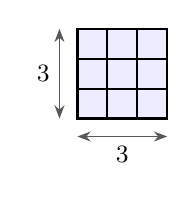
\begin{tikzpicture}[scale=0.38]
  \foreach \x in {0,1,2} \foreach \y in {0,1,2}
    \draw[thick,fill=blue!7] (\x,\y) rectangle ++(1,1);
  \draw[<->,>=Stealth,gray!70!black] (0,-0.6) -- (3,-0.6)
    node[midway,below,font=\small,black] {$3$};
  \draw[<->,>=Stealth,gray!70!black] (-0.6,0) -- (-0.6,3)
    node[midway,left,font=\small,black] {$3$};
\end{tikzpicture}}

% A cube of side 2, divided into the 8 unit cubes that 2 cubed counts.
\newcommand{\cubepic}{%
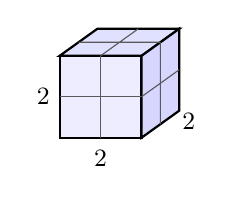
\begin{tikzpicture}[scale=0.52,x={(1cm,0cm)},y={(0.46cm,0.33cm)},z={(0cm,1cm)}]
  \draw[thick,fill=blue!7]  (0,0,0)--(2,0,0)--(2,0,2)--(0,0,2)--cycle;
  \draw[thick,fill=blue!12] (0,0,2)--(2,0,2)--(2,2,2)--(0,2,2)--cycle;
  \draw[thick,fill=blue!16] (2,0,0)--(2,2,0)--(2,2,2)--(2,0,2)--cycle;
  \draw[gray!70!black] (1,0,0)--(1,0,2) (0,0,1)--(2,0,1);
  \draw[gray!70!black] (1,0,2)--(1,2,2) (0,1,2)--(2,1,2);
  \draw[gray!70!black] (2,1,0)--(2,1,2) (2,0,1)--(2,2,1);
  \node[font=\small] at (1,0,-0.5) {$2$};
  \node[font=\small] at (-0.4,0,1) {$2$};
  \node[font=\small] at (2.6,1.2,0) {$2$};
\end{tikzpicture}}

% ----------------------------------------------------------------
% The shapes of the first four dimensions, each drawn with a dot on
% every corner so that the corners can be counted from the picture.
% The dot radius is given in points, so it stays the same size however
% the picture is scaled.
\newcommand{\pointpic}[2]{%
\begin{tikzpicture}[scale=#1]
  \fill[blue!45!black] (0,0) circle (#2);
\end{tikzpicture}}
\newcommand{\linepic}[2]{%
\begin{tikzpicture}[scale=#1]
  \draw[blue!45!black,thick] (0,0)--(2,0);
  \fill[blue!45!black] (0,0) circle (#2) (2,0) circle (#2);
\end{tikzpicture}}
\newcommand{\squarecorners}[2]{%
\begin{tikzpicture}[scale=#1]
  \draw[blue!45!black,thick] (0,0) rectangle (2,2);
  \foreach \a in {0,2} \foreach \b in {0,2} \fill[blue!45!black] (\a,\b) circle (#2);
\end{tikzpicture}}
\newcommand{\cubecorners}[2]{%
\begin{tikzpicture}[scale=#1,x={(1cm,0cm)},y={(0.5cm,0.36cm)},z={(0cm,1cm)},
    line join=round]
  \draw[blue!45!black,thick] (0,0,0)--(2,0,0)--(2,2,0)--(0,2,0)--cycle;
  \draw[blue!45!black,thick] (0,0,2)--(2,0,2)--(2,2,2)--(0,2,2)--cycle;
  \draw[blue!45!black,thick] (0,0,0)--(0,0,2) (2,0,0)--(2,0,2)
    (2,2,0)--(2,2,2) (0,2,0)--(0,2,2);
  \foreach \a in {0,2} \foreach \b in {0,2} \foreach \c in {0,2}
    \fill[blue!45!black] (\a,\b,\c) circle (#2);
\end{tikzpicture}}

% A tesseract, drawn the way a cube is drawn on paper: a small cube
% inside a large cube, with every corner of one joined to the matching
% corner of the other. In four dimensions all eight cubes in the
% picture are the same size and all the joining lines are the same
% length, so the picture stretches the shape in the same way that a
% drawing of a cube stretches its square faces.
\newcommand{\tesspic}[2]{%
\begin{tikzpicture}[scale=#1,x={(1cm,0cm)},y={(0.5cm,0.36cm)},z={(0cm,1cm)},
    line join=round]
  \foreach \a in {0,4} \foreach \b in {0,4} \foreach \c in {0,4}
    \draw[gray!55] (\a,\b,\c) -- ({1+\a/2},{1+\b/2},{1+\c/2});
  \draw[orange!65!black,thick] (1,1,1)--(3,1,1)--(3,3,1)--(1,3,1)--cycle;
  \draw[orange!65!black,thick] (1,1,3)--(3,1,3)--(3,3,3)--(1,3,3)--cycle;
  \draw[orange!65!black,thick] (1,1,1)--(1,1,3) (3,1,1)--(3,1,3)
    (3,3,1)--(3,3,3) (1,3,1)--(1,3,3);
  \draw[blue!45!black,thick] (0,0,0)--(4,0,0)--(4,4,0)--(0,4,0)--cycle;
  \draw[blue!45!black,thick] (0,0,4)--(4,0,4)--(4,4,4)--(0,4,4)--cycle;
  \draw[blue!45!black,thick] (0,0,0)--(0,0,4) (4,0,0)--(4,0,4)
    (4,4,0)--(4,4,4) (0,4,0)--(0,4,4);
  \foreach \a in {0,4} \foreach \b in {0,4} \foreach \c in {0,4} {%
    \fill[blue!45!black] (\a,\b,\c) circle (#2);
    \fill[orange!65!black] ({1+\a/2},{1+\b/2},{1+\c/2}) circle (#2);}
\end{tikzpicture}}

% Characters this language's font has not got are borrowed from another,
% rather than being silently dropped - see docs/translated-sheet-latex.md
\directlua{%
  if luaotfload and luaotfload.add_fallback then
    luaotfload.add_fallback("eallatinfallback",
      { "Noto Serif:mode=harf;" })
  else
    tex.error("this luaotfload is too old to register a fallback font")
  end
}
\usepackage[english]{babel}
\babelprovide[import]{chinese-traditional}
\babelfont[chinese-traditional]{rm}[Renderer=Harfbuzz, BoldFont={Noto Sans CJK TC}, ItalicFont={Noto Sans CJK TC}, BoldItalicFont={Noto Sans CJK TC}, RawFeature={fallback=eallatinfallback}]{Noto Sans CJK TC}
\babelfont[chinese-traditional]{sf}[Renderer=Harfbuzz, BoldFont={Noto Sans CJK TC}, ItalicFont={Noto Sans CJK TC}, BoldItalicFont={Noto Sans CJK TC}, RawFeature={fallback=eallatinfallback}]{Noto Sans CJK TC}
\newcommand{\ealtext}[1]{\foreignlanguage{chinese-traditional}{#1}}
\newcommand{\ealtextblock}[1]{{\raggedright\foreignlanguage{chinese-traditional}{#1}\par}}
% ================================================================
% EAL layout helpers
% ================================================================
\usepackage{xcolor}

\definecolor{ealkeycolour}{RGB}{0,128,0}
\definecolor{ealenglish}{RGB}{0,0,0}
\definecolor{ealtwocolour}{RGB}{112,48,160}

\newsavebox{\ealboxen}
\newsavebox{\ealboxtr}
\newlength{\ealglosswd}
\newlength{\ealglossraise}
\setlength{\ealglossraise}{1.15em}

% a tier 3 word, in English and in translation alike
\newcommand{\ealkey}[1]{\textcolor{ealkeycolour}{#1}}
\newcommand{\ealkeytr}[1]{\textcolor{ealkeycolour}{\ealtext{#1}}}

% One translated word above one English word. Built from kernel
% primitives, never a tabular, which would break wherever the sheet
% loads array, booktabs or tabularx. The box is as wide as the wider of
% the two, so a long translation pushes its neighbours aside instead of
% overlapping them, and it claims its full height so a table row or a
% TikZ node makes room for it.
\newcommand{\ealgloss}[2]{%
  \sbox{\ealboxen}{\ealkey{#1}}%
  \sbox{\ealboxtr}{\small\textcolor{ealtwocolour}{\ealtext{#2}}}%
  \setlength{\ealglosswd}{\wd\ealboxen}%
  \ifdim\wd\ealboxtr>\ealglosswd\setlength{\ealglosswd}{\wd\ealboxtr}\fi
  \leavevmode
  \makebox[\ealglosswd][c]{%
    \makebox[0pt][c]{\usebox{\ealboxen}}%
    \makebox[0pt][c]{\raisebox{\ealglossraise}{\usebox{\ealboxtr}}}%
  }%
}

% opens up line spacing around a block of glosses, so the raised
% translations sit clear of the line above
\newenvironment{ealglossed}{\par\linespread{2.1}\selectfont\ignorespaces}{\par}

% a whole translated sentence above its English counterpart. block level,
% so it does not belong inside a tabular cell
\newcommand{\ealpara}[2]{%
  \par\addvspace{0.5\baselineskip}%
  {\color{ealtwocolour}\ealtextblock{#1}}%
  \penalty200
  {\color{ealenglish}#2\par}%
  \addvspace{0.5\baselineskip}%
}

\begin{document}

\begin{center}
  {\Large\bfseries \ealpara{指數與\ealkeytr{根}}{\ealkey{Indices} and \ealkey{Roots}}}
\end{center}

\begin{keyidea}
\ealpara{一個\ealkeytr{指數}告訴我們一個數自乘了多少次。所以 $5^3$ 表示 $5\times5\times5$。\ealkeytr{指數}的複數形式也是\ealkeytr{指數}。一個\ealkeytr{根}可以還原一個\ealkeytr{指數}。}{An \ealkey{index} tells us how many times a number is multiplied by itself. So $5^3$ means $5\times5\times5$. The plural of index is \ealkey{indices}. A \ealkey{root} undoes an \ealkey{index}.}
\end{keyidea}

\parttitle{1}{\ealpara{數的\ealkeytr{指數}與\ealkeytr{根}}{\ealkey{Indices} and \ealkey{roots} of numbers}}

\begin{minipage}[t]{0.56\linewidth}
\vspace{0pt}
\ealpara{$3^2$ 讀作「$3$ 的\ealkeytr{平方}」。$2^3$ 讀作「$2$ 的\ealkeytr{立方}」。}{$3^2$ is read ``three \ealkey{squared}''. $2^3$ is read ``two \ealkey{cubed}''.}

\vspace{4pt}
\ealpara{一個數的\ealkeytr{平方根}，就是當它（\ealkeytr{平方根}）自乘時，會得到該數的值，所以 $\sqrt{9}=3$。一個數的\ealkeytr{立方根}，就是當三個它相乘時，會得到該數的值，所以 $\sqrt[3]{8}=2$。}{The \ealkey{square root} of a number is the value that gives that number when it (the \ealkey{square root}) is multiplied by itself, so $\sqrt{9}=3$. The \ealkey{cube root} of a number is the value that gives that number when three of them are multiplied together, so $\sqrt[3]{8}=2$.}
\end{minipage}\hfill
\begin{minipage}[t]{0.41\linewidth}
\vspace{0pt}
\centering
\begin{tabular}{@{}c@{\hspace{0.9em}}c@{}}
\squarepic & \cubepic\\[4pt]
{\small $3^2=3\times3=9$} & {\small $2^3=2\times2\times2=8$}\\
\end{tabular}
\end{minipage}

\vspace{2pt}
\begin{notation}{indices and roots}
\ealpara{\ealkeytr{指數}與\ealkeytr{根}}{\ealkey{indices} and \ealkey{roots}}

\ealpara{$a^2=a\times a$ 讀作「$a$ 的\ealkeytr{平方}」；$a^3=a\times a\times a$ 讀作「$a$ 的\ealkeytr{立方}」；$\sqrt{a}$ 是 $a$ 的\ealkeytr{平方根}；$\sqrt[3]{a}$ 是 $a$ 的\ealkeytr{立方根}。例如 $7^2=7\times7=49$，$2^3=2\times2\times2=8$，$\sqrt{49}=7$，$\sqrt[3]{8}=2$。}{$a^2=a\times a$ is read ``$a$ \ealkey{squared}''; $a^3=a\times a\times a$ is read ``$a$ \ealkey{cubed}''; $\sqrt{a}$ is the \ealkey{square root} of $a$; $\sqrt[3]{a}$ is the \ealkey{cube root} of $a$. For example $7^2=7\times7=49$, $2^3=2\times2\times2=8$, $\sqrt{49}=7$, $\sqrt[3]{8}=2$.}

\renewcommand{\arraystretch}{1.4}%
\begin{tabular}{@{}>{\large}p{4.3cm}@{\hspace{0.8em}}p{5.0cm}@{\hspace{0.8em}}l@{}}
$a^2=a\times a$ & ``$a$ \ealkey{squared}'' & for example \; $7^2=7\times7=49$\\
$a^3=a\times a\times a$ & ``$a$ \ealkey{cubed}'' & for example \; $2^3=2\times2\times2=8$\\
$\sqrt{a}$ & the \ealkey{square root} of $a$ & for example \; $\sqrt{49}=7$\\
$\sqrt[3]{a}$ & the \ealkey{cube root} of $a$ & for example \; $\sqrt[3]{8}=2$\\
\end{tabular}

\vspace{2pt}
\ealpara{一個\ealkeytr{指數}會把\ealkeytr{底邊}自乘，而一個\ealkeytr{根}會再次找出\ealkeytr{底邊}。}{An \ealkey{index} multiplies the \ealkey{base} by itself, and a \ealkey{root} finds the \ealkey{base} again.}
\end{notation}

\begin{enumerate}

\item \ealpara{計算左邊每項，並畫線連到右邊的答案。之後用計算機核對答案。}{Work out each calculation on the left and draw a line joining it to its answer on the right. Check your answers on a calculator afterwards.}
\matchup{{$5^2$},{$\sqrt{100}$},{$2^3$},{$0.2^2$},{$\sqrt{0.25}$},{$10^3$},
  {$\sqrt[3]{8}$},{$1.5^2$}}%
  {{$0.5$},{$8$},{$2$},{$25$},{$1000$},{$0.04$},{$2.25$},{$10$}}

\end{enumerate}

\begin{enumerate}[resume]

\newpage{}

\item \ealpara{圖形並非按\ealkeytr{縮放}比例繪製。}{The shapes are not drawn to \ealkey{scale}.}


\begin{enumerate}
  \item \ealpara{一個正方形露台邊長 $6$ m。計算它的\ealkeytr{面積}。}{A square patio has sides of length $6$ m. Work out its \ealkey{area}.}

\vspace{2pt}
\begin{minipage}[t]{0.34\linewidth}
\centering
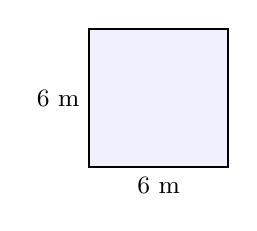
\begin{tikzpicture}[baseline=(current bounding box.north),scale=0.8]
  \draw[thick,fill=blue!6] (0,0) rectangle (2.2,2.2);
  \node[below,font=\small] at (1.1,0) {$6$ m};
  \node[left,font=\small] at (0,1.1) {$6$ m};
\end{tikzpicture}
\end{minipage}%
\begin{minipage}[t]{0.62\linewidth}
\vspace{1.4em}
\begin{ealglossed}
\ealgloss{\ealkey{Area}}{\ealkeytr{面積}} $=6^2=6\times6=\ansline[1.8cm]$ m$^2$
\end{ealglossed}
\end{minipage}

  \item \ealpara{第二個正方形露台的\ealkeytr{面積}是 $144$ m$^2$。計算它其中一條邊的長度。}{A second square patio has an \ealkey{area} of $144$ m$^2$. Work out the length of one of its sides.}

\vspace{2pt}
\begin{minipage}[t]{0.34\linewidth}
\centering
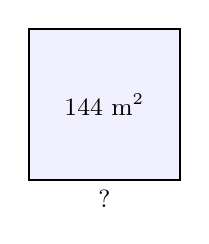
\begin{tikzpicture}[baseline=(current bounding box.north),scale=0.8]
  \draw[thick,fill=blue!6] (0,0) rectangle (2.4,2.4);
  \node[font=\small] at (1.2,1.2) {$144$ m$^2$};
  \node[below,font=\small] at (1.2,0) {$?$};
\end{tikzpicture}
\end{minipage}%
\begin{minipage}[t]{0.62\linewidth}
\vspace{1.4em}
\begin{ealglossed}
Side $=\sqrt{144}=\ansline[1.8cm]$ m
\end{ealglossed}
\end{minipage}

  \item \ealpara{一個儲物箱是一個\ealkeytr{立方}體，\ealkeytr{稜}長 $4$ cm。計算它的\ealkeytr{體積}。}{A storage box is a \ealkey{cube} with \ealkey{edges} of length $4$ cm. Work out its \ealkey{volume}.}

\vspace{2pt}
\begin{minipage}[t]{0.34\linewidth}
\centering
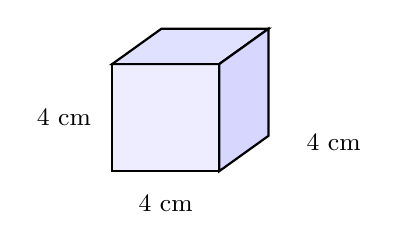
\begin{tikzpicture}[baseline=(current bounding box.north),scale=0.68,
    x={(1cm,0cm)},y={(0.46cm,0.33cm)},z={(0cm,1cm)}]
  \draw[thick,fill=blue!7]  (0,0,0)--(2,0,0)--(2,0,2)--(0,0,2)--cycle;
  \draw[thick,fill=blue!12] (0,0,2)--(2,0,2)--(2,2,2)--(0,2,2)--cycle;
  \draw[thick,fill=blue!16] (2,0,0)--(2,2,0)--(2,2,2)--(2,0,2)--cycle;
  \node[font=\small] at (1,0,-0.6) {$4$ cm};
  \node[font=\small] at (-0.9,0,1) {$4$ cm};
  \node[font=\small] at (3.4,1.6,0) {$4$ cm};
\end{tikzpicture}
\end{minipage}%
\begin{minipage}[t]{0.62\linewidth}
\vspace{1.4em}
\begin{ealglossed}
\ealgloss{\ealkey{Volume}}{\ealkeytr{體積}} $=4^3=\ansline[3.4cm]$ cm$^3$
\end{ealglossed}
\end{minipage}

  \item \ealpara{第二個儲物箱是一個\ealkeytr{立方}體，\ealkeytr{體積}是 $125$ cm$^3$。計算它其中一條\ealkeytr{稜}的長度。}{A second storage box is a \ealkey{cube} with a \ealkey{volume} of $125$ cm$^3$. Work out the length of one of its \ealkey{edges}.}

\vspace{2pt}
\begin{minipage}[t]{0.34\linewidth}
\centering
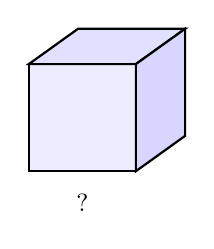
\begin{tikzpicture}[baseline=(current bounding box.north),scale=0.68,
    x={(1cm,0cm)},y={(0.46cm,0.33cm)},z={(0cm,1cm)}]
  \draw[thick,fill=blue!7]  (0,0,0)--(2,0,0)--(2,0,2)--(0,0,2)--cycle;
  \draw[thick,fill=blue!12] (0,0,2)--(2,0,2)--(2,2,2)--(0,2,2)--cycle;
  \draw[thick,fill=blue!16] (2,0,0)--(2,2,0)--(2,2,2)--(2,0,2)--cycle;
  \node[font=\small] at (1,0,-0.6) {$?$};
\end{tikzpicture}

\vspace{1pt}
{\small \ealgloss{Volume}{\ealkeytr{體積}} $=125$ cm$^3$}
\end{minipage}%
\begin{minipage}[t]{0.62\linewidth}
\vspace{1.4em}
\begin{ealglossed}
\ealgloss{\ealkey{Edge}}{\ealkeytr{稜}} $=\ansline[3.4cm]$ cm
\end{ealglossed}
\end{minipage}

  \item \ealpara{一塊正方形地磚的\ealkeytr{面積}是 $0.25$ m$^2$。計算它其中一條邊的長度。}{A square floor tile has an \ealkey{area} of $0.25$ m$^2$. Work out the length of one of its sides.}

\vspace{2pt}
\begin{minipage}[t]{0.34\linewidth}
\centering
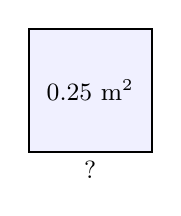
\begin{tikzpicture}[baseline=(current bounding box.north),scale=0.8]
  \draw[thick,fill=blue!6] (0,0) rectangle (1.95,1.95);
  \node[font=\small] at (0.975,0.975) {$0.25$ m$^2$};
  \node[below,font=\small] at (0.975,0) {$?$};
\end{tikzpicture}
\end{minipage}%
\begin{minipage}[t]{0.62\linewidth}
\vspace{1.4em}
\begin{ealglossed}
Side $=\sqrt{0.25}=\ansline[1.8cm]$ m
\end{ealglossed}
\end{minipage}

  \item \ealpara{一個正方形花園的\ealkeytr{面積}是 $50$ m$^2$。不使用計算機，找出其中一條邊的長度介乎哪兩個\ealkeytr{非負整數}之間。解釋你如何知道。}{A square garden has an \ealkey{area} of $50$ m$^2$. Without a calculator, find the two \ealkey{whole numbers} that the length of one side lies between. Explain how you know.}

\vspace{2pt}
\begin{minipage}[t]{0.34\linewidth}
\centering
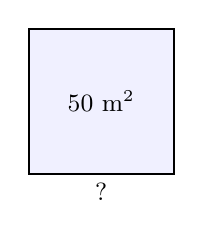
\begin{tikzpicture}[baseline=(current bounding box.north),scale=0.8]
  \draw[thick,fill=blue!6] (0,0) rectangle (2.3,2.3);
  \node[font=\small] at (1.15,1.15) {$50$ m$^2$};
  \node[below,font=\small] at (1.15,0) {$?$};
\end{tikzpicture}
\end{minipage}%
\begin{minipage}[t]{0.62\linewidth}
\vspace{1.4em}
\ealpara{邊長在 \ansline[1.2cm] m 與 \ansline[1.2cm] m 之間，因為}{The side is between \ansline[1.2cm] m and \ansline[1.2cm] m, because}

\vspace{14pt}
\ansline[9.5cm]
\end{minipage}
\end{enumerate}

\end{enumerate}

\vspace{6pt}

\newpage{}

\parttitle{2}{\ealpara{指數與\ealkeytr{代數變數}}{\ealkey{Indices} and \ealkey{algebraic variables}}}

\ealpara{一個\ealkeytr{代數變數}，例如 $a$、$x$ 或 $m$，可以是任何數。就像 $5^3=5\times5\times5$，$a^3$ 表示 $a\times a\times a$。}{An \ealkey{algebraic variable}, such as $a$, $x$ or $m$, could be any number. Just like $5^3=5\times5\times5$, $a^3$ means $a\times a\times a$.}


\begin{warning}
\ealpara{在 $5a^2$ 中，\ealkeytr{指數}只屬於 $a$，所以 $5a^2=5\times a\times a$。它\textbf{不是} $5a\times5a$。如果 $a=2$，那麼 $5a^2=5\times2\times2=20$，但 $5a\times5a=10\times10=100$。}{In $5a^2$ the \ealkey{index} belongs to the $a$ only, so $5a^2=5\times a\times a$. It is \textbf{not} $5a\times5a$. If $a=2$ then $5a^2=5\times2\times2=20$, but $5a\times5a=10\times10=100$.}
\end{warning}

\begin{wex}{writing a fraction in index form}
\ealpara{把分數寫成\ealkeytr{指數形式}。把 $\dfrac{a\times a\times a}{b\times b}$ 寫成\ealkeytr{指數形式}。}{writing a \ealkey{fraction} in \ealkey{index form}. Write $\dfrac{a\times a\times a}{b\times b}$ in \ealkey{index form}.}

\ealpara{第1步：數\ealkeytr{分子}。$a$ 出現 $3$ 次，所以\ealkeytr{分子}是 $a^3$。第2步：數\ealkeytr{分母}。$b$ 出現 $2$ 次，所以\ealkeytr{分母}是 $b^2$。第3步：寫出\ealkeytr{分數}。$\dfrac{a\times a\times a}{b\times b}=\dfrac{a^3}{b^2}$。}{Step 1 --- count the \ealkey{numerator}. $a$ appears $3$ times, so the \ealkey{numerator} is $a^3$. Step 2 --- count the \ealkey{denominator}. $b$ appears $2$ times, so the \ealkey{denominator} is $b^2$. Step 3 --- write the \ealkey{fraction}. $\dfrac{a\times a\times a}{b\times b}=\dfrac{a^3}{b^2}$.}

\small
\smallskip
\renewcommand{\arraystretch}{1.6}
\begin{tabular}{@{}l@{\hspace{1.2em}}l@{}}
\textbf{Step 1 --- count the \ealkey{numerator}.}
  & $a$ appears $3$ times, so the \ealkey{numerator} is $a^3$.\\
\textbf{Step 2 --- count the \ealkey{denominator}.}
  & $b$ appears $2$ times, so the \ealkey{denominator} is $b^2$.\\
\textbf{Step 3 --- write the \ealkey{fraction}.}
  & $\dfrac{a\times a\times a}{b\times b}=\dfrac{a^3}{b^2}$\\
\end{tabular}
\end{wex}


\begin{enumerate}[resume]

\item \ealpara{把每個\ealkeytr{表達式}寫成\ealkeytr{指數形式}。先填寫 (a) 和 (b) 的空格，然後用同樣方法\ealkeytr{化簡}其餘\ealkeytr{表達式}。}{Write each \ealkey{expression} in \ealkey{index form}. Fill in the gaps in parts (a) and (b), then \ealkey{simplify} the remaining \ealkey{expressions} in the same way.}
\begin{enumerate}
  \item $a\times a\times a\times a=a^{\boxgap}$
  \item $\dfrac{c\times c\times c}{d\times d}=\dfrac{c^{\boxgap[7pt]}}{d^{\boxgap[7pt]}}$
\end{enumerate}
\vspace{4pt}
\begin{multicols}{3}
\begin{enumerate}[resume]
  \item $b\times b\times b\times b\times b$
  \item $3\times m\times m$
  \item $\dfrac{p\times p\times p}{q\times q\times q\times q}$
  \item $\dfrac{2\times x\times x\times x}{y\times y}$
  \item $\dfrac{a\times a\times b\times b\times b}{c\times c}$
  \item $\dfrac{t\times t}{5\times u\times u\times u}$
\end{enumerate}
\end{multicols}
\vspace{8em}

\item \ealpara{把每個\ealkeytr{表達式}完整寫成乘法。第一題已為你完成。}{Write each \ealkey{expression} out in full as a multiplication. The first one is done for you.}
\begin{enumerate}
  \item $x^3=x\times x\times x$
\end{enumerate}
\vspace{2pt}
\begin{multicols}{2}
\begin{enumerate}[resume]
  \item $y^5=\ansline[4cm]$
  \item $4t^2=\ansline[4cm]$
  \item $\dfrac{m^2}{n^3}=\ansline[4cm]$
  \item $\dfrac{a^4}{b}=\ansline[4cm]$
\end{enumerate}
\end{multicols}

\end{enumerate}

\vspace{6pt}

\newpage{}

\parttitle{3}{\ealpara{在\ealkeytr{分數}中約去\ealkeytr{因數}}{Cancelling \ealkey{factors} in a \ealkey{fraction}}}

\ealpara{當\ealkeytr{分子}和\ealkeytr{分母}同時除以同一個數時，\ealkeytr{分數}的值保持不變。因此新的\ealkeytr{分數}與原本的是\ealkeytr{等值}。}{A \ealkey{fraction} stays the same value when the \ealkey{numerator} and the \ealkey{denominator} are both divided by the same number. Since the new \ealkey{fraction} is \ealkey{equivalent} to the original.}

\begin{keyidea}
\ealpara{當\ealkeytr{分子}和\ealkeytr{分母}寫成乘法時，同時出現在兩邊的\ealkeytr{因數}可以從兩邊約去。這稱為\ealkeytr{約分}，寫法是把上方和下方的該\ealkeytr{因數}劃掉。}{When the \ealkey{numerator} and the \ealkey{denominator} are written as multiplications, a \ealkey{factor} that appears in both can be divided out of both. This is called \ealkey{cancelling}, and it is written by crossing the \ealkey{factor} out on the top and on the bottom.}
\end{keyidea}

\begin{wex}{simplify $\dfrac{12}{18}$}
\ealpara{\ealkeytr{化簡} $\dfrac{12}{18}$。第1步：把\ealkeytr{分子}和\ealkeytr{分母}寫成乘法。$\dfrac{12}{18}=\dfrac{2\times2\times3}{2\times3\times3}$。第2步：劃掉兩邊都出現的每個\ealkeytr{因數}。$\dfrac{12}{18}=\dfrac{\cancel{2}\times2\times\cancel{3}}{\cancel{2}\times\cancel{3}\times3}$。第3步：把上方和下方剩下的相乘。$\dfrac{12}{18}=\dfrac{2}{3}$。}{\ealkey{Simplify} $\dfrac{12}{18}$. Step 1 --- write the \ealkey{numerator} and the \ealkey{denominator} as multiplications. $\dfrac{12}{18}=\dfrac{2\times2\times3}{2\times3\times3}$. Step 2 --- cross out each \ealkey{factor} that appears in both. $\dfrac{12}{18}=\dfrac{\cancel{2}\times2\times\cancel{3}}{\cancel{2}\times\cancel{3}\times3}$. Step 3 --- multiply what is left on the top and on the bottom. $\dfrac{12}{18}=\dfrac{2}{3}$.}

\small
\renewcommand{\arraystretch}{1.9}
\begin{tabular}{@{}l@{\hspace{1.2em}}l@{}}
\textbf{Step 1 --- write the \ealkey{numerator} and the \ealkey{denominator} as multiplications.}
  & $\dfrac{12}{18}=\dfrac{2\times2\times3}{2\times3\times3}$\\
\textbf{Step 2 --- cross out each \ealkey{factor} that appears in both.}
  & $\dfrac{12}{18}=\dfrac{\cancel{2}\times2\times\cancel{3}}
    {\cancel{2}\times\cancel{3}\times3}$\\
\textbf{Step 3 --- multiply what is left on the top and on the bottom.}
  & $\dfrac{12}{18}=\dfrac{2}{3}$\\
\end{tabular}
\end{wex}

\begin{enumerate}[resume]

\item \ealpara{用\ealkeytr{約分}的方法\ealkeytr{化簡}每個\ealkeytr{分數}。先填寫 (a) 和 (b) 的空格，然後用同樣方法做 (c) 至 (f)。}{\ealkey{Simplify} each \ealkey{fraction} by \ealkey{cancelling}. Fill in the gaps in parts (a) and (b), then do parts (c) to (f) in the same way.}
\begin{enumerate}
  \item $\dfrac{8}{12}=\dfrac{2\times2\times2}{2\times2\times3}
         =\dfrac{\cancel{2}\times\cancel{2}\times2}
          {\cancel{2}\times\cancel{2}\times3}
         =\dfrac{\boxgap[11pt]}{\boxgap[11pt]}$
  \item $\dfrac{15}{25}=\dfrac{5\times3}{5\times\boxgap[11pt]}
         =\dfrac{\boxgap[11pt]}{\boxgap[11pt]}$
\end{enumerate}
\vspace{6pt}
\begin{multicols}{4}
\begin{enumerate}[resume]
  \item $\dfrac{18}{24}$
  \item $\dfrac{14}{21}$
  \item $\dfrac{45}{60}$
  \item $\dfrac{24}{36}$
\end{enumerate}
\end{multicols}
\vspace{6em}

% The list inside multicols does not pass its count on, so the letters
% after (f) are started by hand.
\begin{enumerate}[start=7]
  \item \ealpara{一班 $28$ 名學生中有 $12$ 名步行上學。圖中顯示該班，步行的學生已塗色。把步行上學的學生佔全班的\ealkeytr{分數}寫成\ealkeytr{最簡形式}。}{$12$ of the $28$ pupils in a class walk to school. The picture shows the class, with the pupils who walk shaded. Write the \ealkey{fraction} of the class who walk to school in its \ealkey{simplest form}.}

\vspace{4pt}
\begin{minipage}[t]{0.40\linewidth}
\centering
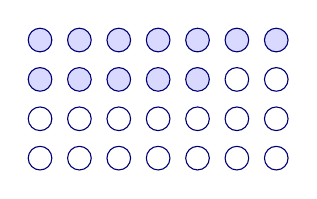
\begin{tikzpicture}[baseline=(current bounding box.north),scale=0.5]
  \foreach \i in {0,...,27} {
    \pgfmathtruncatemacro{\col}{mod(\i,7)}
    \pgfmathtruncatemacro{\row}{\i/7}
    \ifnum\i<12
      \draw[blue!45!black,fill=blue!15] (\col,-\row) circle (0.3);
    \else
      \draw[blue!45!black,fill=white] (\col,-\row) circle (0.3);
    \fi}
\end{tikzpicture}
\end{minipage}%
\begin{minipage}[t]{0.56\linewidth}
\vspace{0.6em}
\ealpara{步行者所佔的\ealkeytr{分數} $=\dfrac{12}{28}=\ansline[3cm]$}{\ealkey{Fraction} who walk $=\dfrac{12}{28}=\ansline[3cm]$}
\end{minipage}

\vspace{3em}
  \item \ealpara{一個蛋糕混合物重 $120$ g，其中 $45$ g 是糖。把糖佔混合物的\ealkeytr{分數}寫成\ealkeytr{最簡形式}。}{A cake mixture weighs $120$ g, and $45$ g of it is sugar. Write the \ealkey{fraction} of the mixture that is sugar in its \ealkey{simplest form}.}

\vspace{5em}
\end{enumerate}

\end{enumerate}


\newpage{}

\ealpara{\ealkeytr{代數變數}會像數一樣\ealkeytr{約分}。當下方的每個\ealkeytr{因數}都約去時，\ealkeytr{分母}是 $1$，不是沒有；\ealkeytr{分母}為 $1$ 的\ealkeytr{分數}等於它的\ealkeytr{分子}。}{\ealkey{Algebraic variables} \ealkey{cancel} in the same way as numbers. When every \ealkey{factor} on the bottom \ealkey{cancels}, the \ealkey{denominator} is $1$, not nothing, a \ealkey{fraction} with a \ealkey{denominator} of $1$ is equal to its \ealkey{numerator}.}

\begin{wex}{cancelling with numbers and variables}
\ealpara{用數和\ealkeytr{代數變數}約分。$\dfrac{a\times a\times a}{a\times a}=\dfrac{\cancel{a}\times\cancel{a}\times a}{\cancel{a}\times\cancel{a}}=\dfrac{a}{1}=a$：下方的每個\ealkeytr{因數}都約去，剩下 $1$。$\dfrac{2\times3\times a\times a}{2\times a}=\dfrac{\cancel{2}\times3\times\cancel{a}\times a}{\cancel{2}\times\cancel{a}}=\dfrac{3\times a}{1}=3a$：數和\ealkeytr{代數變數}分別約去。}{\ealkey{cancelling} with numbers and \ealkey{algebraic variables}. $\dfrac{a\times a\times a}{a\times a}=\dfrac{\cancel{a}\times\cancel{a}\times a}{\cancel{a}\times\cancel{a}}=\dfrac{a}{1}=a$: every \ealkey{factor} on the bottom \ealkey{cancels}, leaving $1$. $\dfrac{2\times3\times a\times a}{2\times a}=\dfrac{\cancel{2}\times3\times\cancel{a}\times a}{\cancel{2}\times\cancel{a}}=\dfrac{3\times a}{1}=3a$: the numbers and the \ealkey{algebraic variables} are \ealkey{cancelled} separately.}

\small
\renewcommand{\arraystretch}{2.2}
\begin{tabular}{@{}l@{\hspace{1.5em}}l@{}}
$\dfrac{a\times a\times a}{a\times a}
  =\dfrac{\cancel{a}\times\cancel{a}\times a}{\cancel{a}\times\cancel{a}}
  =\dfrac{a}{1}=a$
  & every \ealkey{factor} on the bottom \ealkey{cancels}, leaving $1$\\
$\dfrac{2\times3\times a\times a}{2\times a}
  =\dfrac{\cancel{2}\times3\times\cancel{a}\times a}
   {\cancel{2}\times\cancel{a}}=\dfrac{3\times a}{1}=3a$
  & the numbers and the \ealkey{algebraic variables} are \ealkey{cancelled} separately\\
\end{tabular}
\end{wex}

\begin{enumerate}[resume]

\item \ealpara{用\ealkeytr{約分}的方法\ealkeytr{化簡}每個\ealkeytr{分數}，然後把答案寫成\ealkeytr{指數形式}。先填寫 (a) 的空格。}{\ealkey{Simplify} each \ealkey{fraction} by \ealkey{cancelling}, then write the answer in \ealkey{index form}. Fill in the gaps in part (a) first.}
\begin{enumerate}
  \item $\dfrac{a\times a\times a\times a}{a\times a}
         =\dfrac{\cancel{a}\times\cancel{a}\times a\times a}
          {\cancel{a}\times\cancel{a}}=\dfrac{a\times a}{1}=a^{\boxgap}$
\end{enumerate}
\vspace{6pt}
\begin{enumerate}[resume]
  \item $\dfrac{b\times b\times b\times b\times b}{b\times b} =$
  \item $\dfrac{2\times2\times m\times m}{2\times m}=$
  \item $\dfrac{3\times5\times p\times p\times p}{5\times p}=$
  \item $\dfrac{x\times x\times y}{x\times y\times y}=$
  \item $\dfrac{2\times3\times t\times t}{3\times3\times t}=$
  \item $\dfrac{4\times x\times x\times y}{6\times x\times y\times y}=$
  \item $\dfrac{5\times5\times a\times b\times b}{5\times a\times a\times b}=$
  \item \ealpara{Lena \ealkeytr{化簡} $\dfrac{a\times a}{a\times a\times a}$ 並寫下 $a$。解釋 Lena 的錯誤，並寫出正確答案。}{Lena \ealkey{simplifies} $\dfrac{a\times a}{a\times a\times a}$ and writes $a$. Explain the mistake Lena has made, and write down the correct answer.}

\vspace{6pt}
\ansline[16cm]

\vspace{16pt}
\ansline[16cm]
\end{enumerate}
\vspace{10em}

\end{enumerate}

\newpage{}

\parttitle{4}{\ealpara{化簡以\ealkeytr{指數}寫成的\ealkeytr{分數}}{Simplifying \ealkey{fractions} written with \ealkey{indices}}}

\ealpara{以\ealkeytr{指數}寫成的\ealkeytr{分數}也用同樣方法\ealkeytr{化簡}。我們把每個\ealkeytr{次方}完整寫成乘法，約去上方和下方都出現的\ealkeytr{因數}，並把剩下的寫成\ealkeytr{指數形式}。}{A \ealkey{fraction} written with \ealkey{indices} is \ealkey{simplified} in the same way. We write each \ealkey{power} out in full as a multiplication, \ealkey{cancel} the \ealkey{factors} that appear on the top and on the bottom, and write what is left in \ealkey{index form}.}

\begin{wex}{simplifying fractions written with indices}
\ealpara{\ealkeytr{化簡}以\ealkeytr{指數}寫成的\ealkeytr{分數}。$\dfrac{a^5}{a^2}=\dfrac{\cancel{a}\times\cancel{a}\times a\times a\times a}{\cancel{a}\times\cancel{a}}=a^3$：五個 $a$ 中有兩個約去，剩下三個。$\dfrac{6a^3}{2a}=\dfrac{\cancel{2}\times3\times\cancel{a}\times a\times a}{\cancel{2}\times\cancel{a}}=3a^2$：$6=2\times3$，所以\ealkeytr{因數} $2$ 也約去。}{\ealkey{simplifying} \ealkey{fractions} written with \ealkey{indices}. $\dfrac{a^5}{a^2}=\dfrac{\cancel{a}\times\cancel{a}\times a\times a\times a}{\cancel{a}\times\cancel{a}}=a^3$: two of the five $a$s \ealkey{cancel}, leaving three. $\dfrac{6a^3}{2a}=\dfrac{\cancel{2}\times3\times\cancel{a}\times a\times a}{\cancel{2}\times\cancel{a}}=3a^2$: $6=2\times3$, so a \ealkey{factor} of $2$ \ealkey{cancels} as well.}

\small
\renewcommand{\arraystretch}{2.2}
\begin{tabular}{@{}l@{\hspace{2em}}l@{}}
$\dfrac{a^5}{a^2}
  =\dfrac{\cancel{a}\times\cancel{a}\times a\times a\times a}
   {\cancel{a}\times\cancel{a}}=a^3$
  & two of the five $a$s \ealkey{cancel}, leaving three\\
$\dfrac{6a^3}{2a}
  =\dfrac{\cancel{2}\times3\times\cancel{a}\times a\times a}
   {\cancel{2}\times\cancel{a}}=3a^2$
  & $6=2\times3$, so a \ealkey{factor} of $2$ \ealkey{cancels} as well\\
\end{tabular}
\end{wex}

\begin{enumerate}[resume]

\item \ealpara{\ealkeytr{化簡}左邊每個\ealkeytr{分數}。畫線連到右邊的答案。}{\ealkey{Simplify} each \ealkey{fraction} on the left. Draw a line joining it to its answer on the right.}

\vspace{4pt}
\matchup[1.6]{{$\dfrac{a^5}{a^2}$},{$\dfrac{a^2}{a^2}$},{$\dfrac{6a^4}{2a^2}$},
  {$\dfrac{a^3b}{ab}$},{$\dfrac{4a^2}{8a}$},{$\dfrac{a^2b^3}{a^2b}$},
  {$\dfrac{10a^3}{5a^3}$},{$\dfrac{a^6}{a^2}$}}%
  {{$b^2$},{$a^4$},{$2$},{$a^3$},{$\dfrac{a}{2}$},{$1$},{$a^2$},{$3a^2$}}

\end{enumerate}

\newpage

\begin{enumerate}[resume]

\item
\begin{enumerate}
  \item \ealpara{寫出三個不同的\ealkeytr{分數}，它們\ealkeytr{化簡}後都等於 $2a^2$。其中一個的\ealkeytr{分母}必須有不等於 $1$ 的數。}{Write down three different \ealkey{fractions} that \ealkey{simplify} to $2a^2$. One of them must have a number other than $1$ in the \ealkey{denominator}.}

\vspace{12pt}
\ansline[3.4cm]\hfill \ansline[3.4cm]\hfill \ansline[3.4cm]

\vspace{12pt}
  \item \ealpara{用\ealkeytr{代數變數} $a$ 和 $b$ 寫出一個\ealkeytr{分數}（不等於 $\frac{a^2}{b}$），使它\ealkeytr{化簡}後等於 $\frac{a^2}{b}$。}{Write down a \ealkey{fraction} (not equal to $\frac{a^2}{b}$) using the \ealkey{algebraic variables} $a$ and $b$ that \ealkey{simplifies} to $\frac{a^2}{b}$.}

\vspace{16pt}
\ansline[5cm]


\vspace{8pt}
\item \ealpara{用\ealkeytr{代數變數} $x$、$y$ 和 $z$ 寫出一個\ealkeytr{分數}，使它\ealkeytr{化簡}後等於 $\frac{1}{xy^2}$。}{Write down a \ealkey{fraction} using the \ealkey{algebraic variables} $x$, $y$ and $z$ that \ealkey{simplifies} to $\frac{1}{xy^2}$.}

\vspace{16pt}
\ansline[5cm]


\vspace{8pt}
  \item \ealpara{Ben 說 $\frac{3a^2}{3a^2}=0$，因為上方和下方的每個\ealkeytr{因數}都約去，沒有剩下。解釋 Ben 的錯誤，並寫出正確答案。}{Ben says that $\frac{3a^2}{3a^2}=0$, because every \ealkey{factor} on the top and on the bottom \ealkey{cancels} and nothing is left. Explain the mistake Ben has made, and write down the correct answer.}

\vspace{6pt}
\ansline[16cm]

\vspace{16pt}
\ansline[16cm]
\end{enumerate}

\item \ealpara{在這題中，我們找出一個更快的方法來\ealkeytr{化簡}像 $\dfrac{a^7}{a^3}$ 這樣的\ealkeytr{分數}。}{In this question we find a quicker way to \ealkey{simplify} a \ealkey{fraction} such as $\dfrac{a^7}{a^3}$.}
\begin{enumerate}
  \item \ealpara{把每個\ealkeytr{分數}完整寫出並\ealkeytr{約分}來\ealkeytr{化簡}。每個答案用\ealkeytr{指數形式}表示。}{\ealkey{Simplify} each \ealkey{fraction} by writing it out in full and \ealkey{cancelling}. Give each answer in \ealkey{index form}.}

\vspace{8pt}
$\dfrac{a^7}{a^3}=\ansline[2.4cm]$ \hfill $\dfrac{b^9}{b^4}=\ansline[2.4cm]$
\hfill $\dfrac{c^6}{c^5}=\ansline[2.4cm]$

\vspace{3.5em}
  \item \ealpara{觀察每個\ealkeytr{分數}及其答案中的\ealkeytr{指數}。描述一個不用把\ealkeytr{次方}完整寫出就能找到答案的更快方法。}{Look at the \ealkey{indices} in each \ealkey{fraction} and in its answer. Describe a quicker way to find the answer without writing the \ealkey{powers} out in full.}

\vspace{6pt}
\ansline[16cm]

\vspace{16pt}
\ansline[16cm]

\vspace{6pt}
  \item \ealpara{用你更快的方法\ealkeytr{化簡}這些\ealkeytr{分數}。}{Use your quicker way to \ealkey{simplify} these \ealkey{fractions}.}

\vspace{8pt}
$\dfrac{x^{20}}{x^{13}}=\ansline[2.4cm]$ \hspace{3em}
$\dfrac{y^{100}}{y^{99}}=\ansline[2.4cm]$

\vspace{6pt}
  \item \ealpara{對 $\dfrac{a^3}{a^3}$ 使用你更快的方法。\ealkeytr{約分}顯示 $\dfrac{a^3}{a^3}=1$。這暗示 $a^0$ 等於甚麼？}{Use your quicker way on $\dfrac{a^3}{a^3}$. \ealkey{Cancelling} shows that $\dfrac{a^3}{a^3}=1$. What does this suggest $a^0$ is equal to?}

\vspace{10pt}
$\dfrac{a^3}{a^3}=a^{\boxgap}$ \hspace{3em} so \hspace{3em} $a^0=\ansline[2.4cm]$
\end{enumerate}

\end{enumerate}

\newpage{}

\vspace{6pt}

\parttitle{5}{\ealpara{擴展：\ealkeytr{階乘}、\ealkeytr{負}數與第四\ealkeytr{維度}}{Extension: \ealkey{factorials}, \ealkey{negative} numbers and the fourth \ealkey{dimension}}}

\ealpara{一個\ealkeytr{非負整數}的\ealkeytr{階乘}寫成在它後面加一個驚嘆號。\ealkeytr{表達式} $n!$ 表示把從 $n$ 到 $1$ 的每個\ealkeytr{非負整數}相乘，所以 $5!=5\times4\times3\times2\times1=120$。}{The \ealkey{factorial} of a \ealkey{whole number} is written with an exclamation mark after it. The \ealkey{expression} $n!$ means multiply together every \ealkey{whole number} from $n$ down to $1$, so $5!=5\times4\times3\times2\times1=120$.}

$10!=10\times9\times8\times7\times6\times5\times4\times3\times2\times1=3\,628\,800$.

\begin{enumerate}[resume]

\item \ealpara{計算每個\ealkeytr{階乘}。}{Work out each \ealkey{factorial}.}
\begin{multicols}{4}
\begin{enumerate}
  \item $3!=\ansline[1.8cm]$
  \item $4!=\ansline[1.8cm]$
  \item $6!=\ansline[1.8cm]$
  \item $1!=\ansline[1.8cm]$
\end{enumerate}
\end{multicols}

\end{enumerate}

\begin{wex}{simplify $\dfrac{6!}{4!}$}
\ealpara{\ealkeytr{化簡} $\dfrac{6!}{4!}$。兩個\ealkeytr{階乘}都完整寫出。從 $4$ 向下的每個\ealkeytr{非負整數}都在上方和下方出現，所以所有那些\ealkeytr{因數}都約去。}{\ealkey{simplify} $\dfrac{6!}{4!}$. Both \ealkey{factorials} are written out in full. Every \ealkey{whole number} from $4$ downwards appears on the top and on the bottom, so all of those \ealkey{factors} \ealkey{cancel}.}

\small
\smallskip
\[\frac{6!}{4!}
  =\frac{6\times5\times\cancel{4}\times\cancel{3}\times\cancel{2}\times\cancel{1}}
   {\cancel{4}\times\cancel{3}\times\cancel{2}\times\cancel{1}}
  =6\times5=30\]
\end{wex}

\begin{enumerate}[resume]

\item \ealpara{把\ealkeytr{階乘}完整寫出並\ealkeytr{約分}來\ealkeytr{化簡}每個\ealkeytr{表達式}。不要先算出\ealkeytr{階乘}的值。}{\ealkey{Simplify} each \ealkey{expression} by writing the \ealkey{factorials} out in full and \ealkey{cancelling}. Do not work the \ealkey{factorials} out first.}
\begin{multicols}{3}
\begin{enumerate}
  \item $\dfrac{5!}{3!}$
  \item $\dfrac{10!}{9!}$
  \item $\dfrac{8!}{6!}$
  \item $\dfrac{7!}{5!\times2!}$
  \item $\dfrac{100!}{98!}$
  \item $\dfrac{12!}{10!\times2!}$
\end{enumerate}
\end{multicols}
\vspace{9em}

\item \ealpara{對任何大於 $1$ 的\ealkeytr{非負整數} $n$，\ealkeytr{表達式} $\dfrac{n!}{(n-1)!}$ 總是\ealkeytr{化簡}為 $n$。解釋原因。}{For any \ealkey{whole number} $n$ that is greater than $1$, the \ealkey{expression} $\dfrac{n!}{(n-1)!}$ always \ealkey{simplifies} to $n$. Explain why.}

\vspace{6pt}
\ansline[16cm]

\vspace{16pt}
\ansline[16cm]

\vspace{16pt}
\ansline[16cm]

\newpage{}

\item \ealpara{當\ealkeytr{底邊}是\ealkeytr{負}數時，括號表示整個\ealkeytr{負}數自乘，所以 $(-2)^3=(-2)\times(-2)\times(-2)$。}{When the \ealkey{base} is \ealkey{negative}, the brackets show that the whole \ealkey{negative} number is multiplied by itself, so $(-2)^3=(-2)\times(-2)\times(-2)$.}
\begin{enumerate}
  \item \ealpara{完成下表。}{Complete the table.}

\ealpara{表格欄位：\ealkeytr{表達式}、完整寫出、答案。}{Table columns: \ealkey{Expression}, written out in full, \ealkey{Answer}.}

\vspace{2pt}
\begin{center}
\renewcommand{\arraystretch}{1.8}
\begin{tabular}{|>{\centering\arraybackslash}p{2.4cm}|>{\centering\arraybackslash}p{6.4cm}|>{\centering\arraybackslash}p{2.4cm}|}
\hline
\textbf{\ealkey{Expression}} & \textbf{Written out in full} & \textbf{Answer}\\
\hline
$(-2)^2$ & $(-2)\times(-2)$ & $4$\\ \hline
$(-2)^3$ & $(-2)\times(-2)\times(-2)$ & \\ \hline
$(-2)^4$ & & \\ \hline
$(-3)^2$ & & \\ \hline
$(-3)^3$ & & \\ \hline
\end{tabular}
\end{center}

  \item \ealpara{寫下你注意到甚麼：當\ealkeytr{指數}是\ealkeytr{偶數}時，答案的\ealkeytr{正負號}怎樣；當\ealkeytr{指數}是\ealkeytr{奇數}時又怎樣。}{Write down what you notice about the \ealkey{sign} of the answer when the \ealkey{index} is \ealkey{even}, and when the \ealkey{index} is \ealkey{odd}.}

\vspace{6pt}
\ansline[16cm]

\vspace{16pt}
  \item \ealpara{解釋為甚麼會這樣。}{Explain why this happens.}

\vspace{6pt}
\ansline[16cm]
\end{enumerate}

\end{enumerate}


\begin{enumerate}[resume]

\item
\begin{enumerate}
  \item \ealpara{計算 $3\times3$ 和 $(-3)\times(-3)$。寫出兩個自乘後得 $9$ 的數。}{Work out $3\times3$ and $(-3)\times(-3)$. Write down both of the numbers that give $9$ when they are multiplied by themselves.}

\vspace{8pt}
\ansline[5.5cm] \hspace{1.5em} and \hspace{1.5em} \ansline[5.5cm]

\vspace{6pt}
\ealpara{符號 $\sqrt{\phantom{a}}$ 只表示\ealkeytr{正}的\ealkeytr{平方根}，所以 $\sqrt{9}=3$。}{The symbol $\sqrt{\phantom{a}}$ means the \ealkey{positive} \ealkey{square root} only, so $\sqrt{9}=3$.}

\vspace{6pt}
  \item \ealpara{用計算機計算 $\sqrt{-9}$。寫下計算機顯示甚麼，並解釋原因。}{Work out $\sqrt{-9}$ on your calculator. Write down what the calculator shows, and explain why.}

\vspace{6pt}
\ansline[16cm]

\vspace{16pt}
\ansline[16cm]

\vspace{6pt}
  \item \ealpara{計算 $(-2)\times(-2)\times(-2)$。用你的答案寫出 $\sqrt[3]{-8}$。}{Work out $(-2)\times(-2)\times(-2)$. Use your answer to write down $\sqrt[3]{-8}$.}

\vspace{8pt}
\ansline[5.5cm] \hspace{1.5em} so \hspace{1.5em} $\sqrt[3]{-8}=$ \ansline[3cm]

\vspace{6pt}
  \item \ealpara{Sam 說\ealkeytr{負}數的\ealkeytr{根}永遠找不到。用你在 (b) 和 (c) 的答案，說明 Sam 是否正確，並解釋你的答案。}{Sam says that a \ealkey{root} of a \ealkey{negative} number can never be found. Use your answers to parts (b) and (c) to say whether Sam is right, and explain your answer.}

\vspace{6pt}
\ansline[16cm]

\vspace{16pt}
\ansline[16cm]

\end{enumerate}

\item \ealpara{正方形是把一條線沿與自身成\ealkeytr{直角}的方向滑動所得的二維圖形；\ealkeytr{立方}體是把正方形沿與自身成\ealkeytr{直角}的方向滑動所得的三維圖形。\ealkeytr{超立方體}是把\ealkeytr{立方}體沿第四個方向、與自身成\ealkeytr{直角}的方向滑動所得的圖形。我們所居住的空間沒有第四個方向，所以\ealkeytr{超立方體}不能被建造，但仍然可以畫出來，也可以算出它的量度。}{A square is the two-dimensional shape made by sliding a line at \ealkey{right angles} to itself, a \ealkey{cube} is the three-dimensional shape made by sliding a square at \ealkey{right angles} to itself. A \ealkey{tesseract} is the shape made by sliding a \ealkey{cube} at \ealkey{right angles} to itself, in the fourth direction. There is no fourth direction in the space we live in, so a \ealkey{tesseract} cannot be built, but it can still be drawn and its measurements can still be worked out.}

\ealpara{下面是\ealkeytr{超立方體}的圖，也就是我們在三維中能做到的最好畫法。藍色和橙色的角實際上都會是\ealkeytr{超立方體}的外部，而連接內\ealkeytr{立方}體和外\ealkeytr{立方}體的第四類線會與其餘線形成\ealkeytr{直角}（我們沒有足夠的\ealkeytr{維度}來想像這個！）}{Below is a drawing of \ealkey{tesseract}, or the best we can do in three \ealkey{dimensions}. The blue and orange corners would in fact all be the outside of the \ealkey{tesseract}, and the fourth lines connecting the inner and outer \ealkey{cubes} would form \ealkey{right angles} to the remaining lines (we don't have enough \ealkey{dimensions} to imagine this!)}

\vspace{4pt}
\begin{center}
\tesspic{0.82}{2pt}
\end{center}
\vspace{2pt}

\begin{enumerate}
  \item \ealpara{完成下表。數一數每幅圖中的角。}{Complete the table. Count the corners on each picture.}
\nopagebreak

\ealpara{表格欄位：圖形、點、線、正方形、\ealkeytr{立方}體、\ealkeytr{超立方體}；\ealkeytr{維度}、角。}{Table columns: Shape, point, line, square, \ealkey{cube}, \ealkey{tesseract}; \ealkey{Dimensions}, Corners.}

\vspace{2pt}
\begin{center}
\renewcommand{\arraystretch}{1.5}
\begin{tabular}{|l|>{\centering\arraybackslash}p{1.6cm}|>{\centering\arraybackslash}p{1.8cm}|>{\centering\arraybackslash}p{1.9cm}|>{\centering\arraybackslash}p{2.0cm}|>{\centering\arraybackslash}p{2.4cm}|}
\hline
\textbf{Shape} & point & line & square & \ealkey{cube} & \ealkey{tesseract}\\ \hline
\textbf{Picture} & \pointpic{0.4}{3pt} & \linepic{0.45}{3pt}
  & \squarecorners{0.35}{3pt} & \cubecorners{0.35}{3pt}
  & \tesspic{0.28}{1.4pt}\\ \hline
\textbf{\ealkey{Dimensions}} & $0$ & $1$ & $2$ & $3$ & $4$\\ \hline
\textbf{Corners} & $1$ & $2$ & $4$ & & \\ \hline
\end{tabular}
\end{center}

  \item \ealpara{把正方形、\ealkeytr{立方}體和\ealkeytr{超立方體}的角數寫成 $2$ 的\ealkeytr{次方}。}{Write the number of corners of the square, the \ealkey{cube} and the \ealkey{tesseract} as a \ealkey{power} of $2$.}

\vspace{6pt}
Square: \ansline[2.6cm] \hfill Cube: \ansline[2.6cm] \hfill
Tesseract: \ansline[2.6cm]

\vspace{6pt}
  \item \ealpara{\ealkeytr{超立方體}之後的圖形有五個\ealkeytr{維度}。用表中的規律，把它的角數寫成 $2$ 的\ealkeytr{次方}，然後計算出來。}{The shape after the \ealkey{tesseract} has five \ealkey{dimensions}. Use the pattern in the table to write the number of corners it has as a \ealkey{power} of $2$, and then work it out.}

\vspace{10pt}
Corners $=\ansline[3cm]=\ansline[3cm]$

\vspace{6pt}
  \item \ealpara{這個規律中的其中一個圖形有 $1024$ 個角。它有多少個\ealkeytr{維度}？展示你如何知道。}{One of the shapes in this pattern has $1024$ corners. How many \ealkey{dimensions} does it have? Show how you know.}

\vspace{6pt}
\ansline[16cm]

\vspace{16pt}
\ansline[16cm]

\newpage{}

\vspace{6pt}
  \item \ealpara{一個\ealkeytr{稜}長 $3$ cm 的\ealkeytr{立方}體\ealkeytr{體積}是 $3^3=27$ cm$^3$。一個\ealkeytr{稜}長 $3$ cm 的\ealkeytr{超立方體}有\ealkeytr{超體積} $3^4$ cm$^4$。計算 $3^4$。}{A \ealkey{cube} with \ealkey{edges} of length $3$ cm has a \ealkey{volume} of $3^3=27$ cm$^3$. A \ealkey{tesseract} with \ealkey{edges} of length $3$ cm has a \ealkey{hypervolume} of $3^4$ cm$^4$. Work out $3^4$.}

\vspace{10pt}
$3^4=\ansline[6cm]$ cm$^4$

\vspace{6pt}
  \item \ealpara{一個\ealkeytr{超立方體}的\ealkeytr{超體積}是 $16$ cm$^4$。它其中一條\ealkeytr{稜}的長度是 $16$ 的\ealkeytr{四次方根}，寫作 $\sqrt[4]{16}$。找出四個相乘得 $16$ 的數，從而計算 $\sqrt[4]{16}$。}{A \ealkey{tesseract} has a \ealkey{hypervolume} of $16$ cm$^4$. The length of one of its \ealkey{edges} is the \ealkey{fourth root} of $16$, written $\sqrt[4]{16}$. Work out $\sqrt[4]{16}$ by finding the number that gives $16$ when four of them are multiplied together.}

\vspace{10pt}
$\sqrt[4]{16}=\ansline[6cm]$ cm

\vspace{6pt}
  \item \ealpara{證明 $(-2)^4=16$ 也成立。解釋為甚麼\ealkeytr{超立方體}的\ealkeytr{稜}仍然必須是 $2$ cm。}{Show that $(-2)^4=16$ as well. Explain why the \ealkey{edge} of the \ealkey{tesseract} must still be $2$ cm.}

\vspace{6pt}
\ansline[16cm]

\vspace{16pt}
\ansline[16cm]

\vspace{6pt}
  \item \ealpara{第二個\ealkeytr{超立方體}的\ealkeytr{超體積}是 $81$ cm$^4$。計算它其中一條\ealkeytr{稜}的長度。}{A second \ealkey{tesseract} has a \ealkey{hypervolume} of $81$ cm$^4$. Work out the length of one of its \ealkey{edges}.}

\vspace{10pt}
$\sqrt[4]{81}=\ansline[6cm]$ cm

\vspace{6pt}
  \item \ealpara{正方形有 $4$ 條\ealkeytr{稜}，\ealkeytr{立方}體有 $12$ 條\ealkeytr{稜}，\ealkeytr{超立方體}有 $32$ 條\ealkeytr{稜}。\ealkeytr{立方}體的 $12$ 條\ealkeytr{稜}可以寫成 $3\times2^2$。用同樣方式，把正方形的\ealkeytr{稜}數和\ealkeytr{超立方體}的\ealkeytr{稜}數寫成一個數乘以 $2$ 的\ealkeytr{次方}。然後用規律預測五\ealkeytr{維度}圖形有多少條\ealkeytr{稜}。}{A square has $4$ \ealkey{edges}, a \ealkey{cube} has $12$ \ealkey{edges} and a \ealkey{tesseract} has $32$ \ealkey{edges}. The $12$ \ealkey{edges} of a \ealkey{cube} can be written as $3\times2^2$. Write the \ealkey{edges} of a square and the \ealkey{edges} of a \ealkey{tesseract} in the same way, as a number multiplied by a \ealkey{power} of $2$. Then use the pattern to predict how many \ealkey{edges} the five-\ealkey{dimensional} shape has.}

\vspace{6pt}
Square: $4=\ansline[3cm]$ \hfill Cube: $12=3\times2^2$ \hfill
Tesseract: $32=\ansline[3cm]$

\vspace{12pt}
\ansline[16cm]

\vspace{16pt}
\ansline[16cm]

\vspace{6pt}
  \item \ealpara{用這兩個規律，找出六\ealkeytr{維度}圖形的角數和\ealkeytr{稜}數。}{Use both patterns to find the number of corners and the number of \ealkey{edges} of the six-\ealkey{dimensional} shape.}

\vspace{10pt}
Corners $=\ansline[4cm]$ \hfill Edges $=\ansline[4cm]$
\end{enumerate}

\end{enumerate}

\newpage

\heading{\ealpara{答案}{Answers}}

{\small
\begin{multicols}{2}
\raggedcolumns
\setlength{\parskip}{4pt}

\textbf{Q1.} 1--D ($25$) \quad 2--H ($10$) \quad 3--B ($8$) \quad
4--F ($0.04$) \quad 5--A ($0.5$) \quad 6--E ($1000$) \quad 7--C ($2$) \quad
8--G ($2.25$)

\ealpara{\textbf{Q2.} (a) $6\times6=36$ m$^2$ (b) $\sqrt{144}=12$ m (c) $4\times4\times4=64$ cm$^3$ (d) $\sqrt[3]{125}=5$ cm (e) $\sqrt{0.25}=0.5$ m (f) 在 $7$ m 與 $8$ m 之間，因為 $7^2=49$ 且 $8^2=64$，而 $50$ 在 $49$ 與 $64$ 之間。}{\textbf{Q2.} (a) $6\times6=36$ m$^2$ \quad (b) $\sqrt{144}=12$ m \quad (c) $4\times4\times4=64$ cm$^3$ \quad (d) $\sqrt[3]{125}=5$ cm \quad (e) $\sqrt{0.25}=0.5$ m \quad (f) Between $7$ m and $8$ m, because $7^2=49$ and $8^2=64$, and $50$ is between $49$ and $64$.}

\textbf{Q3.} (a) $a^4$ \quad (b) $\dfrac{c^3}{d^2}$ \quad (c) $b^5$ \quad
(d) $3m^2$ \quad (e) $\dfrac{p^3}{q^4}$ \quad (f) $\dfrac{2x^3}{y^2}$ \quad
(g) $\dfrac{a^2b^3}{c^2}$ \quad (h) $\dfrac{t^2}{5u^3}$

\textbf{Q4.} (b) $y\times y\times y\times y\times y$ \quad
(c) $4\times t\times t$ \quad (d) $\dfrac{m\times m}{n\times n\times n}$ \quad
(e) $\dfrac{a\times a\times a\times a}{b}$

\textbf{Q5.} (a) $\dfrac{2}{3}$ \quad
(b) $\dfrac{5\times3}{5\times5}=\dfrac{3}{5}$ \quad (c) $\dfrac{3}{4}$ \quad
(d) $\dfrac{2}{3}$ \quad (e) $\dfrac{3}{4}$ \quad (f) $\dfrac{2}{3}$ \quad
(g) $\dfrac{12}{28}=\dfrac{3}{7}$ \quad (h) $\dfrac{45}{120}=\dfrac{3}{8}$

\textbf{Q6.} (a) $a^2$ \quad (b) $b^3$ \quad (c) $2m$ \quad (d) $3p^2$ \quad
(e) $\dfrac{x}{y}$ \quad (f) $\dfrac{2t}{3}$ \quad (g) $\dfrac{2x}{3y}$
\quad (h) $\dfrac{5b}{a}$ \quad (i) Two $a$s \ealkey{cancel} from the top and the
bottom, which leaves $1$ on the top and one $a$ on the bottom. Lena has put the
$a$ that is left on the top. The answer is $\dfrac{1}{a}$.

\ealpara{\textbf{Q8.} (a) 有很多答案，例如 $\dfrac{2a^3}{a}$、$\dfrac{4a^3}{2a}$ 和 $\dfrac{6a^5}{3a^3}$。(b) 有很多答案，例如 $\dfrac{a^3}{ab}$ 或 $\dfrac{a^2b}{b^2}$。(c) 有很多答案，例如 $\dfrac{z}{xy^2z}$ 或 $\dfrac{xz}{x^2y^2z}$。(d) \ealkeytr{約分}是用同一個\ealkeytr{因數}去除上方和下方，而一個數除以自己是 $1$，不是 $0$。上方剩下的是 $1$，下方剩下的是 $1$，所以 $\dfrac{3a^2}{3a^2}=\dfrac{1}{1}=1$。}{\textbf{Q8.} (a) There are many answers, for example $\dfrac{2a^3}{a}$, $\dfrac{4a^3}{2a}$ and $\dfrac{6a^5}{3a^3}$. \quad (b) There are many answers, for example $\dfrac{a^3}{ab}$ or $\dfrac{a^2b}{b^2}$. \quad (c) There are many answers, for example $\dfrac{z}{xy^2z}$ or $\dfrac{xz}{x^2y^2z}$. \quad (d) \ealkey{Cancelling} divides the top and the bottom by the same \ealkey{factor}, and a number divided by itself is $1$, not $0$. What is left on the top is $1$ and what is left on the bottom is $1$, so $\dfrac{3a^2}{3a^2}=\dfrac{1}{1}=1$.}

\ealpara{\textbf{Q9.} (a) $a^4$、$b^5$、$c$ (b) 用上方的\ealkeytr{指數}減去下方的\ealkeytr{指數}，並保留相同的\ealkeytr{底邊}。(c) $x^7$、$y$ (d) $\dfrac{a^3}{a^3}=a^{3-3}=a^0$，而\ealkeytr{約分}得到 $1$，所以 $a^0=1$。}{\textbf{Q9.} (a) $a^4$, $b^5$, $c$ \quad (b) Subtract the \ealkey{index} on the bottom from the \ealkey{index} on the top, and keep the same \ealkey{base}. \quad (c) $x^7$, $y$ \quad (d) $\dfrac{a^3}{a^3}=a^{3-3}=a^0$, and \ealkey{cancelling} gives $1$, so $a^0=1$.}

\textbf{Q10.} (a) $6$ \quad (b) $24$ \quad (c) $720$ \quad (d) $1$

\textbf{Q11.} (a) $5\times4=20$ \quad (b) $10$ \quad (c) $8\times7=56$ \quad
(d) $\dfrac{7\times6}{2\times1}=21$ \quad (e) $100\times99=9900$ \quad
(f) $\dfrac{12\times11}{2\times1}=66$

\ealpara{\textbf{Q12.} $n!=n\times(n-1)\times(n-2)\times\cdots\times1$ 且 $(n-1)!=(n-1)\times(n-2)\times\cdots\times1$。$(n-1)!$ 的每個\ealkeytr{因數}也都出現在 $n!$ 中，所以它們全都約去。上方唯一剩下的\ealkeytr{因數}是 $n$，而下方是 $1$。}{\textbf{Q12.} $n!=n\times(n-1)\times(n-2)\times\cdots\times1$ and $(n-1)!=(n-1)\times(n-2)\times\cdots\times1$. Every \ealkey{factor} of $(n-1)!$ also appears in $n!$, so all of them \ealkey{cancel}. The only \ealkey{factor} left on the top is $n$, and the bottom is $1$.}

\ealpara{\textbf{Q13.} (a) $(-2)^3=-8$；$(-2)^4=(-2)\times(-2)\times(-2)\times(-2)=16$；$(-3)^2=(-3)\times(-3)=9$；$(-3)^3=(-3)\times(-3)\times(-3)=-27$。(b) \ealkeytr{偶數}的\ealkeytr{指數}給出\ealkeytr{正}答案，\ealkeytr{奇數}的\ealkeytr{指數}給出\ealkeytr{負}答案。(c) 兩個\ealkeytr{負}數相乘給出\ealkeytr{正}答案，所以\ealkeytr{負}號會成對抵消。\ealkeytr{偶數}的\ealkeytr{指數}不會剩下\ealkeytr{負}號，而\ealkeytr{奇數}的\ealkeytr{指數}會剩下一個\ealkeytr{負}號。}{\textbf{Q13.} (a) $(-2)^3=-8$; $(-2)^4=(-2)\times(-2)\times(-2)\times(-2)=16$; $(-3)^2=(-3)\times(-3)=9$; $(-3)^3=(-3)\times(-3)\times(-3)=-27$. \quad (b) An \ealkey{even} \ealkey{index} gives a \ealkey{positive} answer and an \ealkey{odd} \ealkey{index} gives a \ealkey{negative} answer. \quad (c) Two \ealkey{negative} numbers multiplied together give a \ealkey{positive} answer, so the \ealkey{negative} \ealkey{signs} pair up. An \ealkey{even} \ealkey{index} leaves no \ealkey{negative} \ealkey{sign} over, and an \ealkey{odd} \ealkey{index} leaves one \ealkey{negative} \ealkey{sign} over.}

\ealpara{\textbf{Q14.} (a) $3\times3=9$ 且 $(-3)\times(-3)=9$，所以兩個數是 $3$ 和 $-3$。(b) 計算機顯示錯誤。沒有任何數自乘會給出\ealkeytr{負}答案，因為\ealkeytr{正}數乘\ealkeytr{正}數是\ealkeytr{正}數，而\ealkeytr{負}數乘\ealkeytr{負}數也是\ealkeytr{正}數。(c) $(-2)\times(-2)\times(-2)=-8$，所以 $\sqrt[3]{-8}=-2$。(d) Sam 不正確。\ealkeytr{負}數沒有\ealkeytr{平方根}，因為\ealkeytr{偶數}的\ealkeytr{指數}總是給出\ealkeytr{正}答案，但它有\ealkeytr{立方根}，因為\ealkeytr{奇數}的\ealkeytr{指數}可以給出\ealkeytr{負}答案。}{\textbf{Q14.} (a) $3\times3=9$ and $(-3)\times(-3)=9$, so the two numbers are $3$ and $-3$. \quad (b) The calculator shows an error. No number multiplied by itself gives a \ealkey{negative} answer, because a \ealkey{positive} multiplied by a \ealkey{positive} is \ealkey{positive}, and a \ealkey{negative} multiplied by a \ealkey{negative} is also \ealkey{positive}. \quad (c) $(-2)\times(-2)\times(-2)=-8$, so $\sqrt[3]{-8}=-2$. \quad (d) Sam is not right. A \ealkey{negative} number has no \ealkey{square root}, because an \ealkey{even} \ealkey{index} always gives a \ealkey{positive} answer, but it does have a \ealkey{cube root}, because an \ealkey{odd} \ealkey{index} can give a \ealkey{negative} answer.}

\ealpara{\textbf{Q15.} (a) \ealkeytr{立方}體有 $8$ 個角，\ealkeytr{超立方體}有 $16$ 個角。(b) 正方形：$4=2^2$；\ealkeytr{立方}體：$8=2^3$；\ealkeytr{超立方體}：$16=2^4$。\ealkeytr{指數}就是\ealkeytr{維度}的數目。(c) $2^5=32$ 個角 (d) $1024=2^{10}$，所以它有 $10$ 個\ealkeytr{維度}。(e) $3^4=3\times3\times3\times3=81$ cm$^4$ (f) $\sqrt[4]{16}=2$ cm，因為 $2\times2\times2\times2=16$。(g) $(-2)\times(-2)\times(-2)\times(-2)=16$，因為\ealkeytr{指數}是\ealkeytr{偶數}。\ealkeytr{稜}仍然必須是 $2$ cm，因為長度不能是\ealkeytr{負}數。(h) $\sqrt[4]{81}=3$ cm，因為 $3\times3\times3\times3=81$。(i) 正方形：$4=2\times2^1$；\ealkeytr{超立方體}：$32=4\times2^3$。前面的數是\ealkeytr{維度}的數目，而\ealkeytr{指數}比它少一，所以五\ealkeytr{維度}圖形有 $5\times2^4=80$ 條\ealkeytr{稜}。(j) 角 $=2^6=64$；\ealkeytr{稜} $=6\times2^5=192$。}{\textbf{Q15.} (a) The \ealkey{cube} has $8$ corners and the \ealkey{tesseract} has $16$ corners. \quad (b) Square: $4=2^2$; \ealkey{cube}: $8=2^3$; \ealkey{tesseract}: $16=2^4$. The \ealkey{index} is the number of \ealkey{dimensions}. \quad (c) $2^5=32$ corners \quad (d) $1024=2^{10}$, so it has $10$ \ealkey{dimensions}. \quad (e) $3^4=3\times3\times3\times3=81$ cm$^4$ \quad (f) $\sqrt[4]{16}=2$ cm, because $2\times2\times2\times2=16$. \quad (g) $(-2)\times(-2)\times(-2)\times(-2)=16$, because the \ealkey{index} is \ealkey{even}. The \ealkey{edge} must still be $2$ cm, because a length cannot be \ealkey{negative}. \quad (h) $\sqrt[4]{81}=3$ cm, because $3\times3\times3\times3=81$. \quad (i) Square: $4=2\times2^1$; \ealkey{tesseract}: $32=4\times2^3$. The number in front is the number of \ealkey{dimensions} and the \ealkey{index} is one less than it, so the five-\ealkey{dimensional} shape has $5\times2^4=80$ \ealkey{edges}. \quad (j) Corners $=2^6=64$; \ealkey{edges} $=6\times2^5=192$.}

\end{multicols}
}

\end{document}